\documentclass[../main.tex]{subfiles} % Due to use of package subfiles

%%%%%%%%%%%%%%%%%%%%%%%%%%%%%%%%%%%%%%%%%%%%%%%%%%%%%%%%%%%%%%%%%%%%%%%%%%%%%%%%

\begin{document}

\chapter{Confinement in the Lattice Schwinger Model} \label{chap:Confinement}
% Alternative title ''Schwinger model and confinement''

\ldots



\section{QED, QCD, and confinement}

\lipsum[1-3]


%%%%%

\begin{figure}[t]
    \centering
    \begin{tikzpicture}
        % Include the image
        \node[anchor=south west, inner sep=0] (image) at (0, 0) {
            \ifthenelse{\boolean{book}}{
                % Image remains the same size in book as in report class
                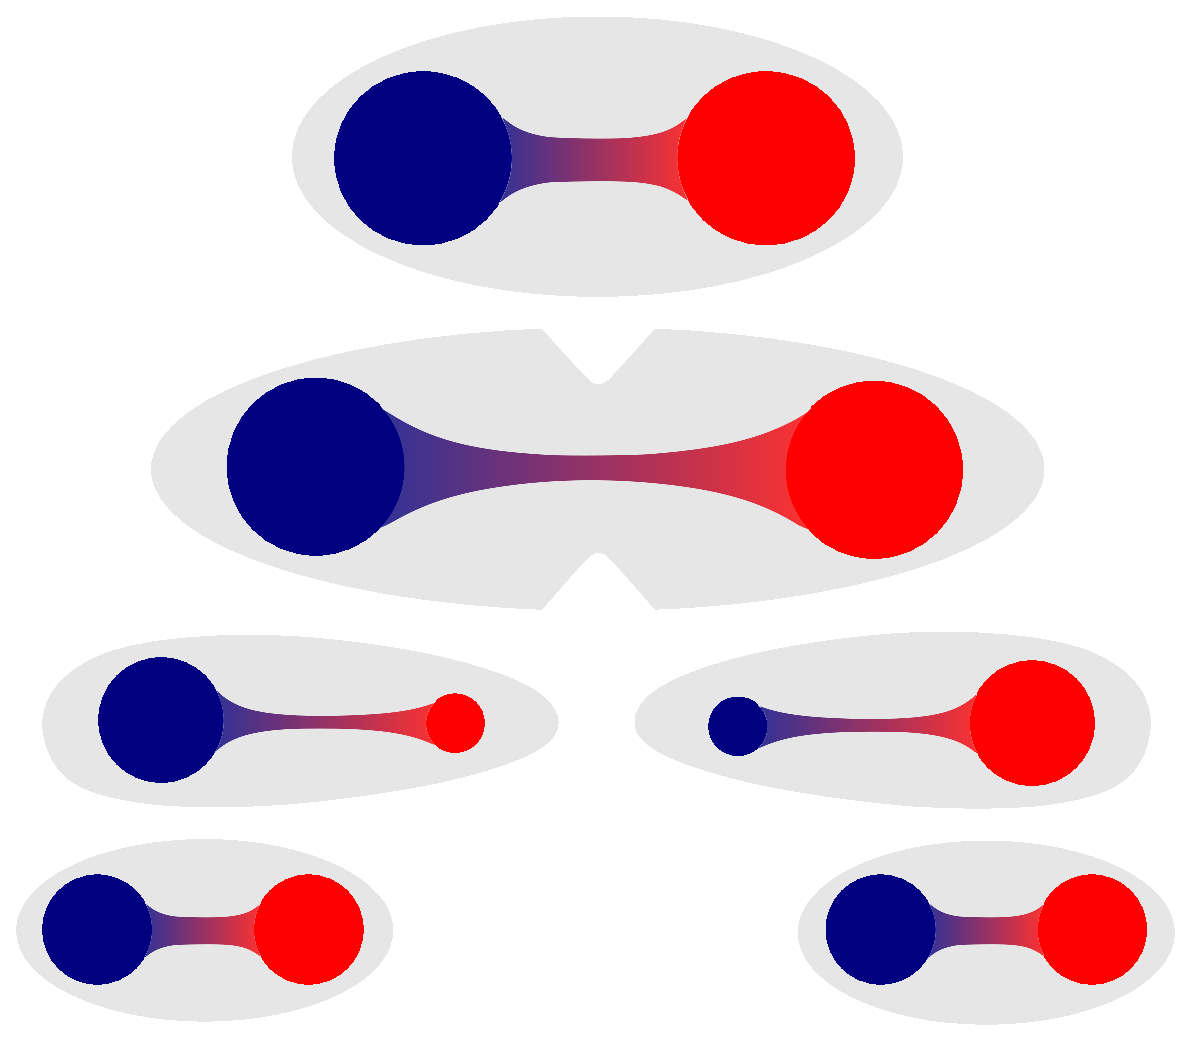
\includegraphics[width=0.7\textwidth]{images/QuarkConfinement.eps}
            }{
                % Size of image in report class
                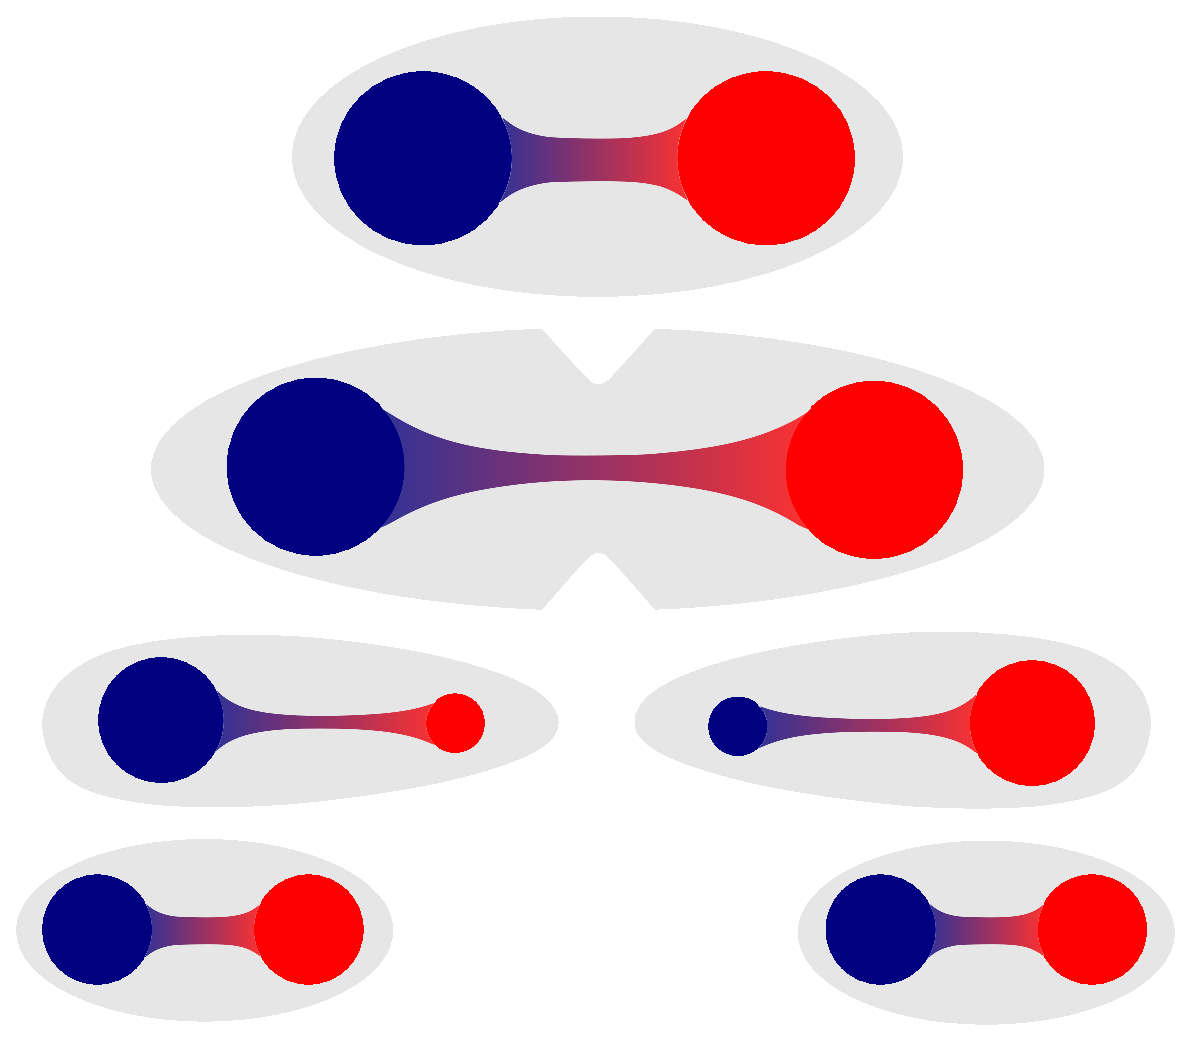
\includegraphics[width=0.8\textwidth]{images/QuarkConfinement.eps}
            }
        };
        % Draw the coordinate system
        \begin{scope}[x={(image.south east)},y={(image.north west)}]
            \draw[thick,|-|] (0.35, 1.03) -- node[above, midway] {\large $r$} (0.65, 1.03);
            \draw[thick,->] (0, 1) -- node[right, midway] {\large time} (0, 0.8);
        \end{scope}
    \end{tikzpicture}
    \caption{As a quark\index{quark} (red) and an antiquark\index{antiquark} (blue) in a meson\index{meson} are pulled away from each other (distance $r$ increases), the energy needed increases until the string tension of the flux tube\index{flux tube} (blue to red gradient) between the particles is sufficient enough, thus the flux tube break, known as string breaking\index{string breaking}, and the energy stored in the flux tube creates a new quark and antiquark such that there is now two mesons. That a quark and an antiquark can never exist on its own is know as colour confinement\index{colour confinement}\index{confinement|see{colour confinement}}. Inspired by Ref. \cite{institutoDeFisicaCorpuscular_numericalApproach_2016}.}
    \label{fig:QuarkConfinement}
\end{figure}

%%%%%



\subsection{Lattice Schwinger model exhibiting confinement} \label{sec:qIsChangeShowed}

\ldots

\cref{eq:LatticeSchwingerModelHamiltonianSpin}
\begin{align}
    H &= a \sum_n \left[ (-1)^{n+1} \frac{m}{2} \sigma_n^z - \frac{1}{2a} \left( \sigma_n^+ S_n^+ \sigma_{n+1}^- + \mathrm{h.c.} \right) + \frac{a^2 q^2 S^2}{2} \left( S_n^z \right)^2 \right]
\end{align}

\cref{eq:GeneratorU(1)SymmetryDiscretized} changes to become
\begin{align}
    G_n = \frac{E_n - E_{n-1}}{a} - q \psi_n\dagger \psi_n - \frac{(-1)^n - 1}{2} \: ,
\end{align}
\begin{align} \label{eq:GeneratorU(1)Symmetry}
    G_n = - S_n^z + S_{n-1}^z - \frac{q}{2} \big( - \sigma_n + (-1)^n \big) \: ,
\end{align}
for $S=1$. \cite{buyens_confinementAndStringBreaking_2016}

\begin{table}[t]
    \centering
    \begin{tabular}{|c|c|c|}
        \hline
        State & \multicolumn{2}{c|}{$G_n / q$} \\
         & Even $n$ & Odd $n$ \\ \hline
        $\ket{\, 0_g\, 0_m\, 0_g}$ & $0$ & $1$ \\ \hline
        $\ket{\, 0_g\, 1_m\, 0_g}$ & $-1$ & $0$ \\ \hline
        $\ket{\, 0_g\, 0_m\, 1_g}$ & $-1$ & $0$ \\ \hline
        $\ket{\, 0_g\, 1_m\, 1_g}$ & $-2$ & $-1$ \\ \hline
        $\ket{\, 0_g\, 0_m\, 2_g}$ & $-2$ & $-1$ \\ \hline
        $\ket{\, 0_g\, 1_m\, 2_g}$ & $-3$ & $-2$ \\ \hline
        $\ket{\, 1_g\, 0_m\, 0_g}$ & $1$ & $2$ \\ \hline
        $\ket{\, 1_g\, 1_m\, 0_g}$ & $0$ & $1$ \\ \hline
        $\ket{\, 1_g\, 0_m\, 1_g}$ & $0$ & $1$ \\ \hline
        \multicolumn{3}{|c|}{\textsl{continued to the right}} \\ \hline
    \end{tabular}
    \hfill
    \begin{tabular}{|c|c|c|}
        \hline
        State & \multicolumn{2}{c|}{$G_n / q$} \\
         & Even $n$ & Odd $n$ \\ \hline
        \multicolumn{3}{|c|}{\textsl{continued from the left}} \\ \hline
        $\ket{\, 1_g\, 1_m\, 1_g}$ & $-1$ & $0$ \\ \hline
        $\ket{\, 1_g\, 0_m\, 2_g}$ & $-1$ & $0$ \\ \hline
        $\ket{\, 1_g\, 1_m\, 2_g}$ & $-2$ & $-1$ \\ \hline
        $\ket{\, 2_g\, 0_m\, 0_g}$ & $2$ & $3$ \\ \hline
        $\ket{\, 2_g\, 1_m\, 0_g}$ & $1$ & $2$ \\ \hline
        $\ket{\, 2_g\, 0_m\, 1_g}$ & $1$ & $2$ \\ \hline
        $\ket{\, 2_g\, 1_m\, 1_g}$ & $0$ & $1$ \\ \hline
        $\ket{\, 2_g\, 0_m\, 2_g}$ & $0$ & $1$ \\ \hline
        $\ket{\, 2_g\, 1_m\, 2_g}$ & $-1$ & $0$ \\ \hline
    \end{tabular}
    \caption{The eigenvalues of the generator from \cref{eq:GeneratorU(1)Symmetry} for the 18 configurations of two gauge fields (denoted with a $g$) with spin-$1$ and the matter field (denoted with an $m$) with spin-\half between them.}
    \label{tab:EigenvaluesOfGenerator}
\end{table}




% MÅL FOR BACHELORPROJEKT NUMERISK DEL
% * Potential eller kraft som funktion af afstand
% * Der kan ikke eksistere en quark uden en antiquark og vice versa
% * Afstand eller energi for hvilken string breaking sker




\end{document}